%%%%%%%%%%%%%%%%%%%%%%%%%%%%%%%%%%%%%%%%%
% LaTeX Template
% http://www.LaTeXTemplates.com
%
% Original author:
% Linux and Unix Users Group at Virginia Tech Wiki 
% (https://vtluug.org/wiki/Example_LaTeX_chem_lab_report)
%
% License:
% CC BY-NC-SA 3.0 (http://creativecommons.org/licenses/by-nc-sa/3.0/)
%
%%%%%%%%%%%%%%%%%%%%%%%%%%%%%%%%%%%%%%%%%

%----------------------------------------------------------------------------------------
%	PACKAGES AND DOCUMENT CONFIGURATIONS
%----------------------------------------------------------------------------------------

\documentclass[11pt]{article}
\usepackage{geometry} % Pour passer au format A4
\geometry{hmargin=0.5cm, vmargin=0.5cm} % 

\usepackage{graphicx} % Required for including pictures
\usepackage{float} % 

%Français
\usepackage[T1]{fontenc} 
\usepackage[english,francais]{babel}
\usepackage[utf8]{inputenc}
\usepackage{eurosym}
\usepackage{lmodern}
\usepackage{url}
\usepackage{multicol}

%Maths
\usepackage{amsmath,amsfonts,amssymb,amsthm}
%\usepackage[linesnumbered, ruled, vlined]{algorithm2e}
%\SetAlFnt{\small\sffamily}

%Autres
\linespread{1} % Line spacing
\setlength\parindent{0pt} % Removes all indentation from paragraphs

\renewcommand{\labelenumi}{\alph{enumi}.} % 
\pagestyle{empty}
%----------------------------------------------------------------------------------------
%	DOCUMENT INFORMATION
%----------------------------------------------------------------------------------------
\begin{document}

%\maketitle % Insert the title, author and date

\setlength{\columnseprule}{1pt}

\textbf{Nom(s), Prénom(s) :}

\begin{multicols}{2}


  \begin{enumerate}
  \item[EX1] Soient $A(2; -4)$ et $B(-2, 4)$ deux points du plan.

    \begin{enumerate}
    \item Soit la droite $(D_1)$ d'équation $(D_1) : 2y + 3x + 5 = 0$. Vérifier si les points $A$ et $B$ appartiennent à $(D_1)$.
    \item Trouver l'équation de la droite $(D_2)$ passant par $A$ et $B$.
    \end{enumerate}

  \item[EX2] Soient le point $C(1, 5)$ et la droite $(D_3) : y = 2x + 5$.

    \begin{enumerate}
    \item Vérifier que $C$ n'appartient par à la droite $(D_3)$.
    \item Trouver l'équation de la droite $(D_4)$ passant par $C$ et parallèle à $(D_3)$.
    \end{enumerate}

  \item[EX3] Soient les droites $(D_3) : y = 2x + 5$ et $(D_5) : y = 3x + 5$.

    \begin{enumerate}
    \item Justifier que les droites $D_5$ et $D_3$ ne sont pas parallèles.
    \item Trouver les coordonnées du point $E$ situé à l'intersectiion de ces deux droites.
    \item Donner l'équation de la droite verticale passant par $E$.
    \item Donner l'équation de la droite horizontale passant par $E$.
    \end{enumerate}


  \item[EX4] Placer les points $A$,$B$, $C$ et $E$. Tracer les droites $(D_1)$, $(D_2)$, $(D_3)$, $(D_4)$ et $(D_5)$.
  \end{enumerate}

  \begin{figure}[H]
    \centering
    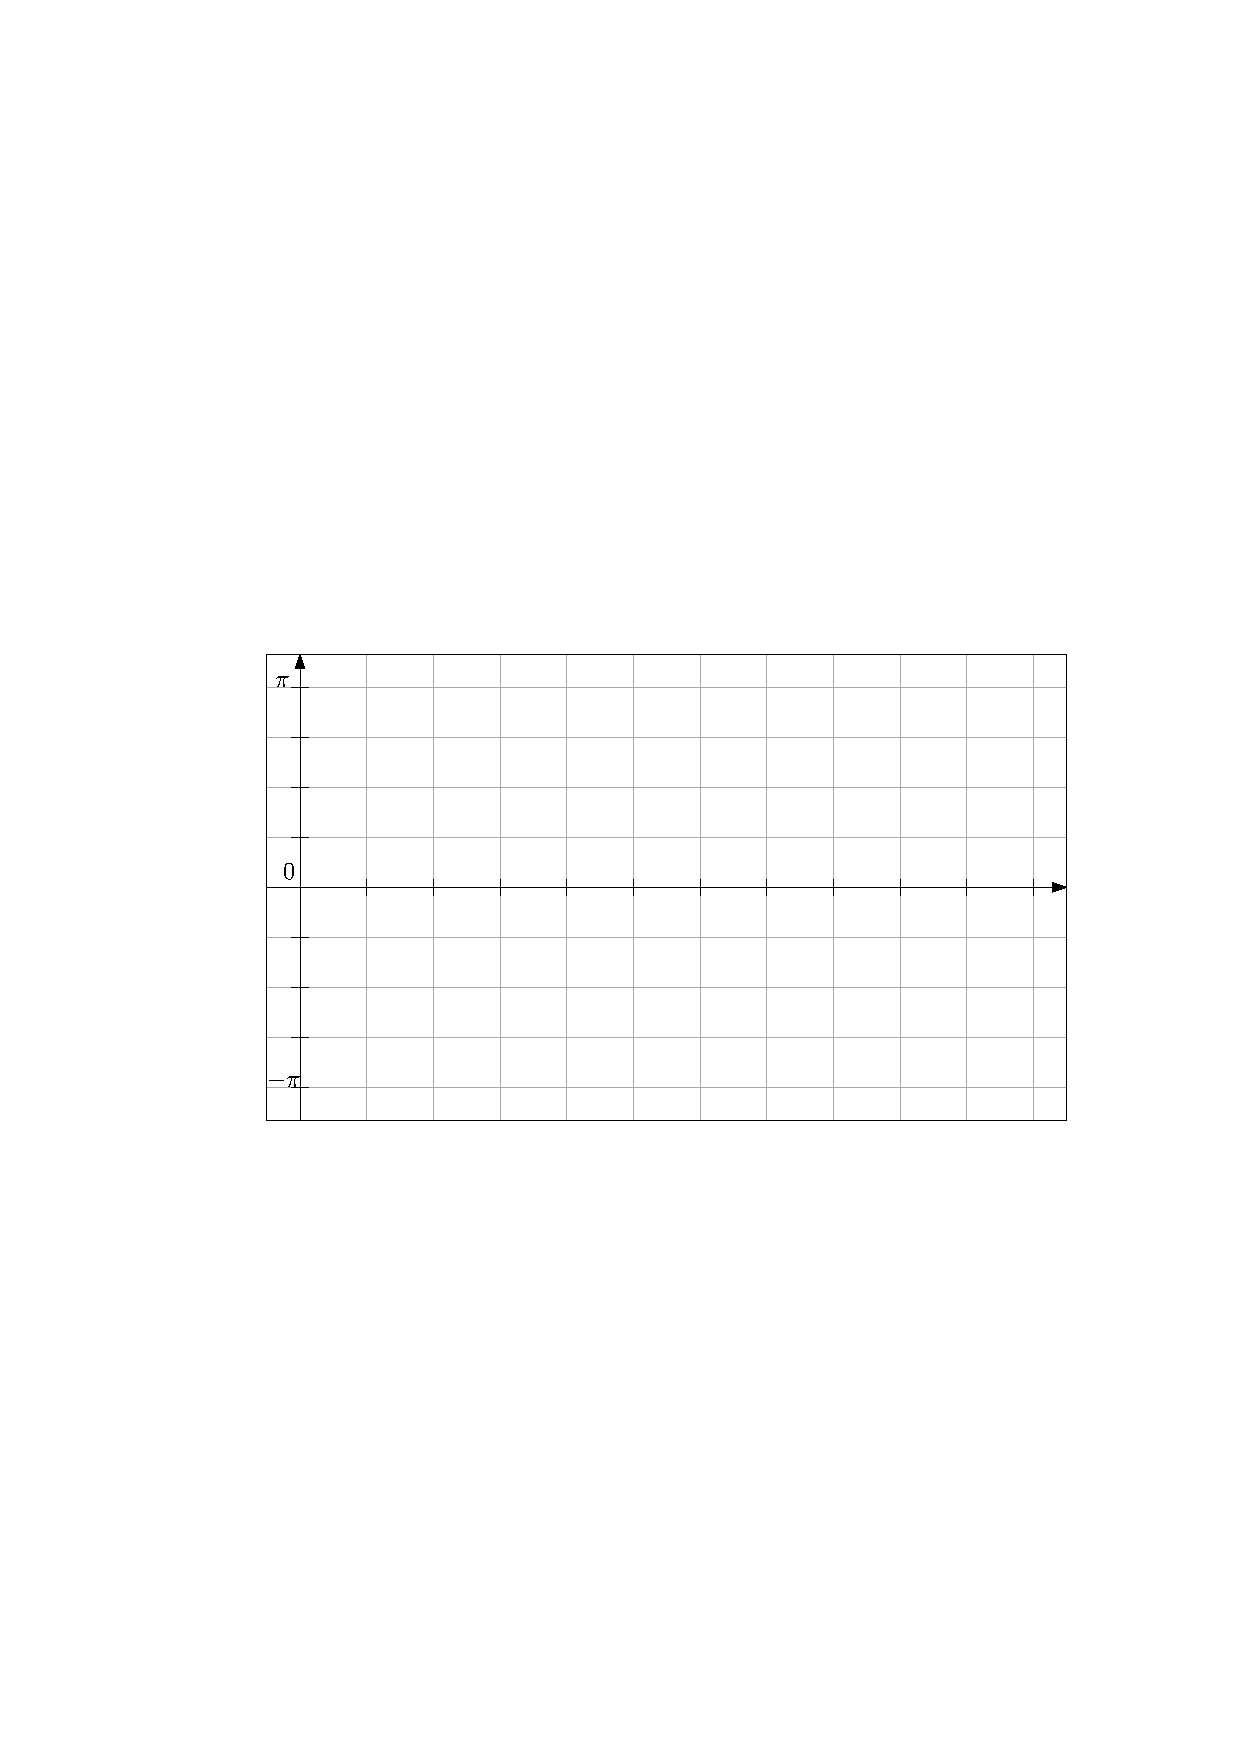
\includegraphics[width=0.8\linewidth]{sources/ie/grille.pdf}
  \end{figure}

\end{multicols}
\end{document}
